%EKG-7 Realisierung/Prozessoreinheit

\subsection{Prozessoreinheit}

Dieses Kapitel gibt eine ausführliche Beschreibung zur Software des Projektes und deren Entwicklung. Zuerst wird der Begriff \textit{State Machine} im Allgemeinen beschrieben. Anschließend wird auf die Implementierung der \textit{State Machine} im Projekt mit der Beschreibung jedes Zustandes eingegangen, sowie auf essenzielle Module und Funktionsprinzipien.  

\subsubsection{State Machine}

Eine \textit{State Machine} ist ein Verhaltensmodell der Softwareentwicklung mit einer endlichen Anzahl von Zuständen. Zwischen diesen Zuständen kann gemäß der Programmlogik oder der Eingangsdaten gewechselt werden.

Eine \textit{State Machine} hat in der Regel einen Initialisierungszustand, in dem die Programmmodule gestartet werden. Der folgende Programmablauf ist von dem Initialisierungszustand abhängig. Nach einer erfolgreichen Initialisierung wird beispielsweise der reguläre Programmablauf fortgeführt. Sollte es bei der Initialisierung zu Fehlern kommen, wird ein Zustand eingenommen indem z.B. mögliche Fehlerursachen angezeigt oder das komplette System abgeschaltet wird. Die Überwachung von Fehlfunktionen findet auch in allen anderen Zuständen statt.

\subsubsection{Zustände der \textit{State Machine}}

In diesem Projekt sind sechs verschiedene Zustände für das EKG-Gerät entwickelt, sowie eine regelmäßige Abfrage der globalen Flags, die jede Sekunde stattfindet. Die Zustände der \textit{State Machine} sind: 
\begin{itemize}
    \item Initialisierung – SYS\_INIT
    \item Leerlauf – IDLE\_STATE
    \item Aufnahme des Kurzzeit-EKG – ECG\_SHORT
    \item Aufnahme des Langzeit-EKG – ECG\_LONG
    \item Stromsparmodus – ENERGY\_SAVING\_MODE
    \item Wakeup Modus – SYS\_WAKEUP
\end{itemize} 
Aus dem Bild ist die Funktionsweise der \textit{State Machine} zu entnehmen. Auf den genauen Ablaub wird in der Beschreibung der einzelnen Zustände eingegangen.
\begin{figure} [!h]
    \centering
    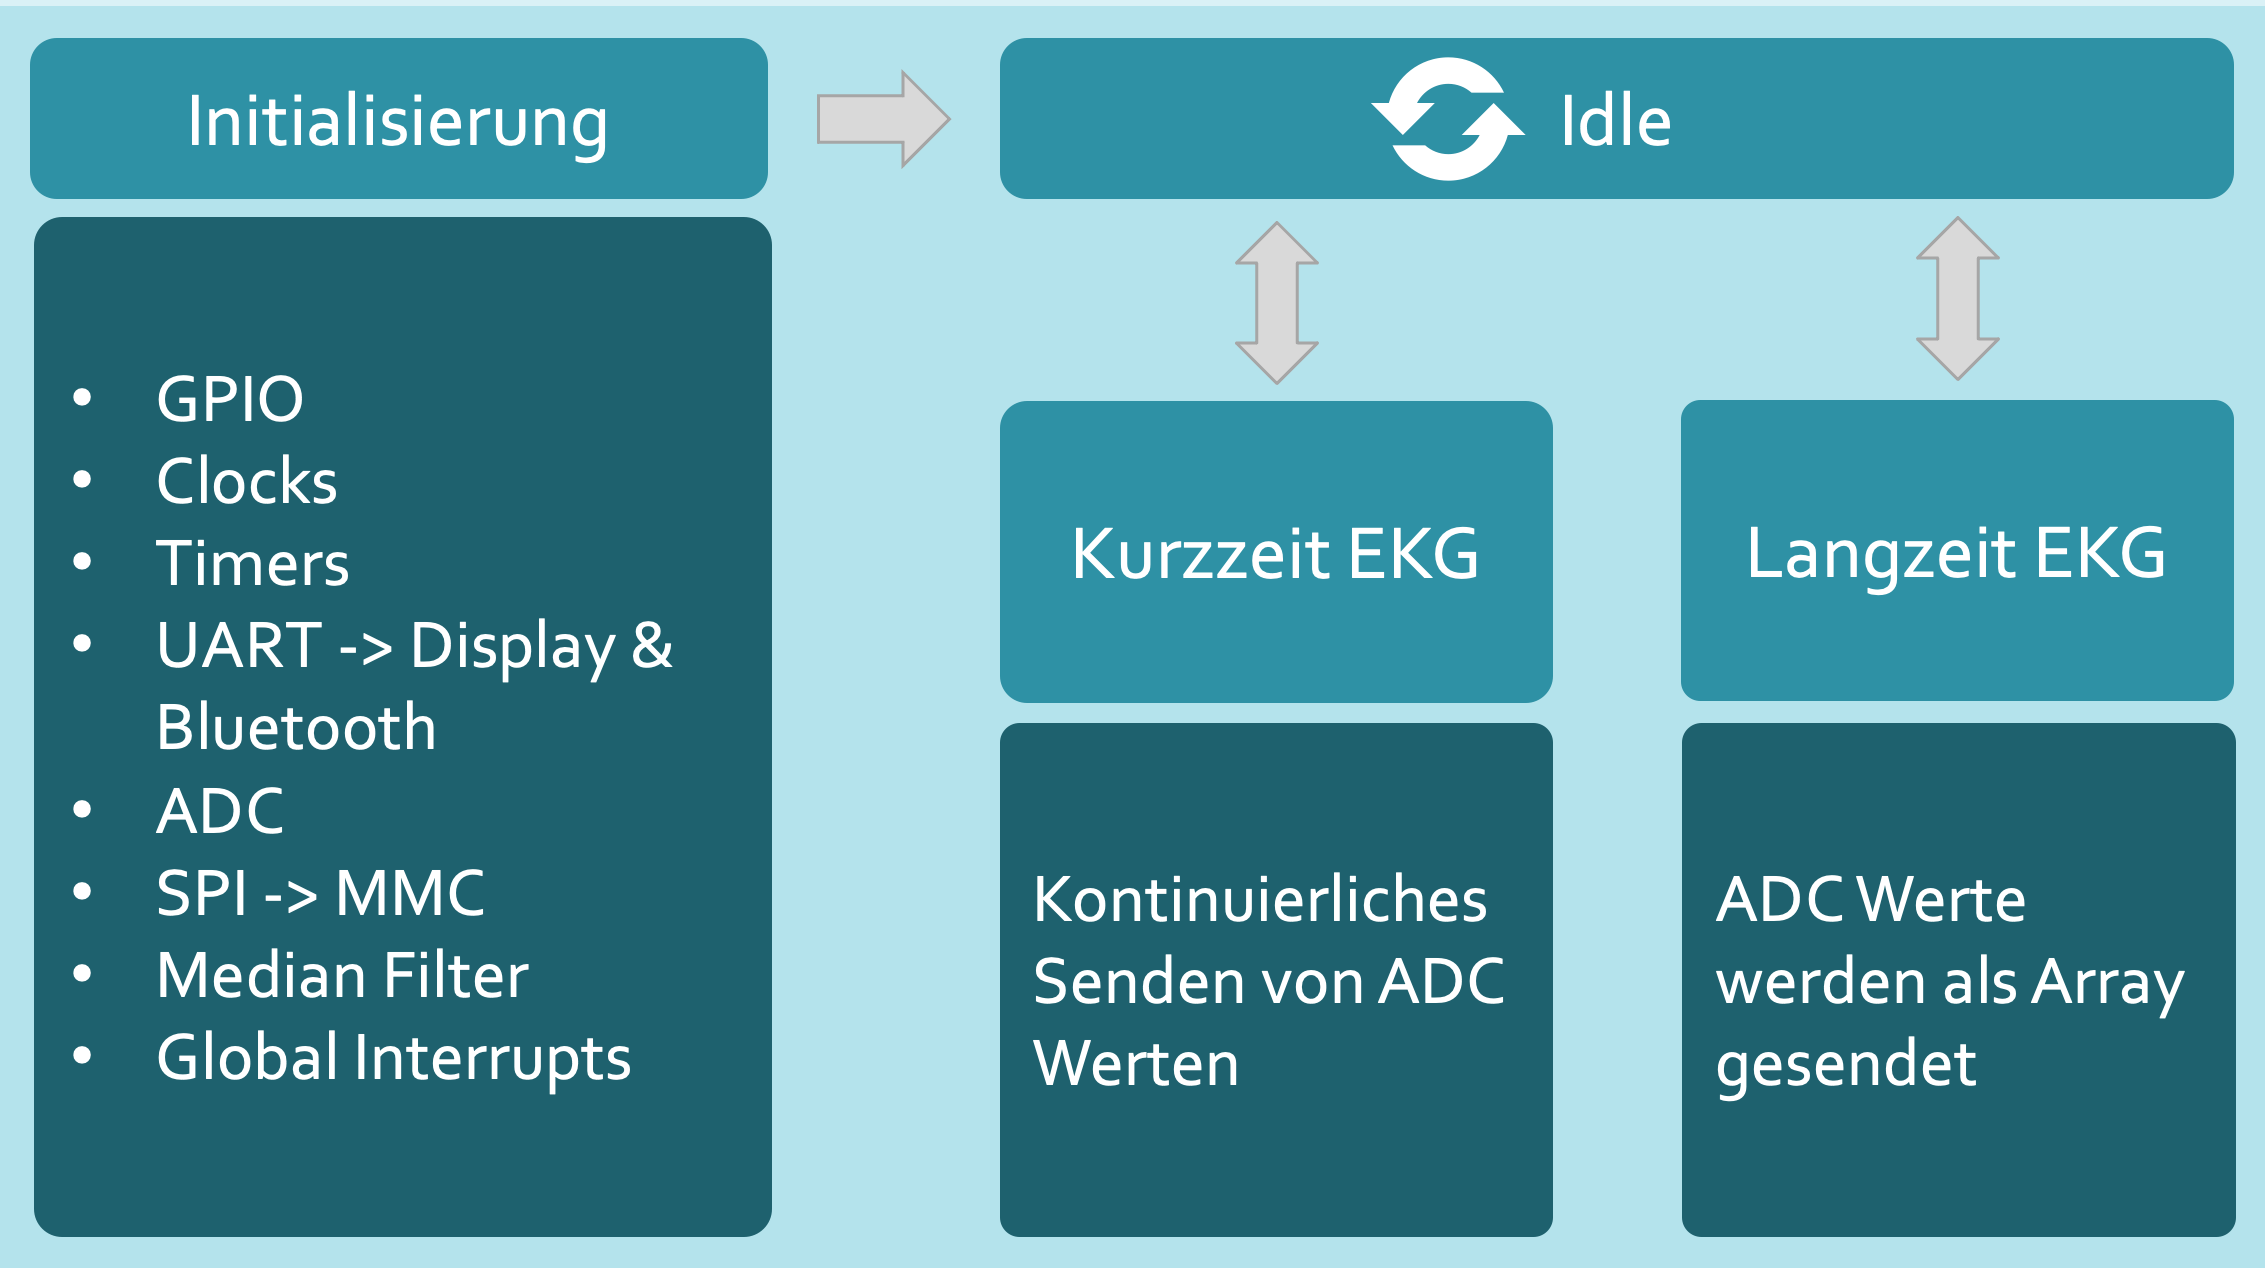
\includegraphics[width=12cm] {State Machine.png}
    \caption{\textit{State Machine} des EKG7}
\end{figure}

\subsubsection{Globale Flags}

Für das Anzeigen diverser Zustände sind in der Software globale \textit{Flags} implementiert. Die \textit{Flags} können folgende Ereignisse widerspiegeln:
\begin{itemize}
    \item Auftreten eines \textit{Interrupts}
    \item Eingang von Daten
    \item Aktueller Zustand der \textit{State Machine}
    \item Betätigen des \textit{Power-Buttons}
    \item Zustände der Module (z.B. aktiv / inaktiv)
    \item \textit{Timer-Interrupt}
    \item Zustand der Bluetooth-Verbindung
    \item Verbindung mit SD-Karte
\end{itemize} 

\subsubsection{Interrupts}

Ein Interrupt ist ein Signal an die MCU, das hardware- oder softwareseitig auftritt und eine sofortige Reaktion der MCU benötigt. Der normale Programmablauf wird dabei gestoppt und zunächst die Befehle der ISR ausgeführt. Nach dem Abarbeiten eines \textit{Interrupts} kehrt die MCU zurück zum normalen Programmablauf.
In dem Projekt werden \textit{Interrupts} für folgende Module verwendet:
\begin{itemize}
    \item GPIO – beim Betätigen der Taste am Gehäuse, Ein- und Ausschalten des Bluetooth Moduls und Einsetzen bzw. Entfernen der SD-Karte
    \item Timer – es treten drei \textit{Interrupts} mit jeweils 1 Hz, 250 Hz und 1 kHz Frequenz auf
    \item UART – beim Empfang von Befehlen vom Display
    \item ADC – beim Empfang von EKG-Signalen und Akkuspannung
\end{itemize} 

\subsubsection{Initialisierung}

Initialisierung oder SYS\_INIT ist der Anfangszustand der MCU nach dem Einschalten. Dieser Zustand ruft die Initialisierungsfunktion aller verwendeten Modulen auf und wird danach verlassen. 

%Hier folgt die Reihenfolge der Module, die im Programm initialisiert werden:
%\begin{itemize}

 %   \item Clocks – ;
 %   \item Timer – 
 %   \item UART – Schnittstelle für Display- und Bluetooth-Verbindung;
 %   \item ADC – Digitalisierung der analogen Signale;
 %   \item SPI – Schnittstelle für Verbindung mit SD-Kartenmodul;
 %   \item FAT – File Allocation Table ist die Dateizuordnungstabelle bzw. ein Dateisystem für die Datenübertragung auf SD-Karte;
 %   \item UART-BT – Kommunikation der MCU mit dem Bluetooth Modul;
 %   \item Median Filter – Filterung der Artefakte bei der Herzfrequenzberechnung;
 %   \item Globle Interrupts – Freischalten der globalen Interrupts.
%\end{itemize}

Im Folgenden wird eine detaillierte Beschreibung von den zu initialisierenden Modulen aufgelistet:
\begin{enumerate}
    \item Watchdog Timer: Ist dem Totmann-Schalter ähnlich. Die MCU wird zurückgesetzt, wenn das Programm ihn nicht explizit ausschaltet
    \item GPIO: General Purpose Input Output ist ein Modul, das die vorhandenen Pins als Inputs oder Outputs initialisiert. Da ihre Funktionalität in aderen Modulen verwendet wird, müssen sie als erstes initialisiert werden. Es werden folgende GPIO-Pins initialisiert:
    \begin{itemize}
        \item LEDs auf der Platine
        \item Buzzer
        \item 5 V-DC/DC enable
        \item Gehäusetaste
        \item Bluetooth-Verbindungszustand
        \item \textit{Card Detect} Pin für das SD-Kartenmodul
    \end{itemize}
    \item Clocks: Es werden drei \textit{Clocks}  für den Mikrocontroller initialisiert. MCLK und SMCLK weisen eine Frequenz von 20 MHz auf. ACLK ist mit einer Frequenz von 32 kHz initialisiert.
    MCLK wird als Taktquelle für die MCU verwendet. SMCLK ist ein Hochfrequenztakt und wird für Peripheriemodule verwendet. ACLK wird für Peripheriemodule verwendet, die einen niederfrequenten Takt benötigen.
    \item Timer: Die \textit{Timer} lösen in gewissen Zeitintervalen \textit{Interrupts} aus. Im Code sind drei \textit{Timer} initialisiert. \textit{Timer} A0 bezieht seinen Takt von SMCLK und hat eine Frequenz von 1 kHz. \textit{Timer} A1 hat ACLK als Taktgeber und wird mit einer Frequenz von 1 Hz aufgerufen. Timer A2 ist an SMCLK gebunden und weist eine Frequenz von 250 Hz auf. Die drei \textit{Timer} funktionieren unabhängig voneinander und haben ihre eigene ISR.
    \item UART Display: Bei der Initialisierung der UART Verbindung zum Display, werden zunächst die Input- (RX) und Output- (TX) Pins festgelegt. Die Frequenz der MCU beträgt 20 MHz und als Baudrate wurde 115200 $s^{-1}$ gewählt. Damit eine Verbindung der beiden Module hergestellt werden kann, muss die Baudrate sowohl beim Display als auch bei der MCU einprogrammiert werden.\\
    Befehle vom Display an die MCU werden mittels \textit{Interrupts} realisiert. Das Display sendet eine Folge zwischen vier und sieben Bytes. Sobald die MCU eine gesendete Byte-Folge erkennt, werden in einem \textit{Interrupt Flags} gesetzt. Anhand dieser \textit{Flags} werden im späteren Verlauf gewisse Funktion auf der MCU aufgerufen.\\
    Bei Befehlen, die von der MCU an das Display gesendet werden, wird im Wesentlichen mit drei Funktionen gearbeitet. Bei der ersten Funktion wird ein Befehl mit der entsprechenden Variablen als \textit{String} (z.B. „page0.akku.val“) an das Display gesendet. Mit der zweiten Funktion wird der dazugehörende Wert, zum Beispiel \textit{akku\_percentage}, von einem \textit{Integer} Wert in einen \textit{String} umgewandelt und anschließend an das Display sendet. Um einen Befehl abzuschließen, erwartet das Display drei Bytes mit dem Inhalt „0xFF“ am Ende. Diese drei Bytes werden in der dritten UART-Funktion an das Display gesendet.
    \item UART Bluetooth-Modul: Das verwendete Bluetooth Modul HC-05 wird über UART angesprochen, wobei die Baudrate 38400 $s^{-1}$ beträgt. Seitens der MCU wird das Hardware-Modul USCI\_A1 verwendet, welches mit Ausnahme der Basisadresse identisch zu USCI\_A0 bzw. Display initialisiert wird.\\
    Um beim Versenden der Nachrichten keine Verzögerung oder zusätzliche CPU Last zu verursachen, wird \textit{Direct Memory Access} (DMA) verwendet. Das DMA-Modul kann automatische Daten im Hintergrund in das TX Register des UART Moduls kopieren. Hierfür wird nach jedem Trigger die Information byteweise übertragen. Als Trigger wird das \textit{Interrupt Flag} UCA1TXIFG gewählt, welches immer dann aktiv ist, wenn das UART Modul bereit ist ein weiteres Byte zu senden.\\
    Damit ein ganzer \textit{String} verschickt werden kann, inktementiert das DMA Modul die Quelladresse nach jedem versendeten Byte. Somit wird nach Aktivierung des Moduls durch setzen des DMA-Enable-Bits ein kompletter String im Hintergrund Byte für Byte versendet, bis die vorgegebene Datengröße abgearbeitet ist und das Enable-Bit automatisch zurückgesetzt wird. Die CPU selbst wird dabei jeweils nur für zwei Takte durch das DMA Modul unterbrochen und muss nicht auf den Abschluss jedes Sendevorgangs warten.
    \item ADC: Danach wird das ADC Modul initialisiert und die beiden Pins für die EKG-Aufnahme und Akkuüberwachung konfiguriert. Als positive Referenzspannungsquelle wird AVCC (3V) für beide ADC Kanäle eingestellt. Negative Referenzspannungsquelle ist AVSS, was dem Massepotential auf der Platine entspricht. Beide Kanäle werden mit ACLK betrieben. Zum Schluss wird der \textit{Interrupt} für dieses Modul aktiviert.
    \item SPI: Die SPI Schnittstelle dient zur Kommunikation mit dem SD-Kartenmodul und wird mit der SMCLK betrieben. Nach dem die gewünschte Frequenz eingestellt wurde, werden die \textit{Interrupts} freigeschaltet, das \textit{Chip Select} Signal an den \textit{Slave} gesendet und der TX Buffer aktiviert.
    \item FAT: Als Kommunikationsprotokoll für FAT, wird die Schnittstelle SPI verwendet. Das FAT-Modul ist für die Initialisierung der SD-Karte verantwortlich. Dafür wird in diesem Projekt eine \textit{Open Source Library} verwendet.
    \item Medianfilter: Der Medianfilter dient dazu, Ausreißer (verursacht durch Bewegungsartefakte des Anwenders) der berechneten Herzfrequenz herauszufiltern. In der Initialisierung wird ein Array mit elf Elementen angelegt, dass als Speicher des Filters dient. Aus diesem Speicher wird nach jeder neuen Pulsberechnung der Median gebildet und ans Display gesendet. Im Gegensatz zu einem Mittelwertfilter haben vereinzelte Ausreißer keinen Einfluss auf das Ergebnis.
\end{enumerate}

\subsubsection{Idle State}

Direkt nach dem Initialisierungsvorgang der MCU wechselt sie in den \textit{IDLE\_STATE} (Leerlauf des Programms). 
Hier wird kontinuierlich abgefragt, ob der Marker für ein Kurz- oder Langzeit-EKG gesetzt ist. Der Marker wird im \textit{Interrupt} gesetzt, der ausgelöst wird nachdem der Benutzer die Aufnahme des EKG startet.
Sobald der Benutzer den Befehl gibt, wird eine CSV Datei auf der SD-Karte erstellt und der Zustand der \textit{State Machine} wechselt entsprechend der gewünschten Aufnahmemethode.

\subsubsection{Kurzzeit-EKG}

Im Falle einer Kurzzeit-Aufnahme startet man das EKG auf dem Display im Unterpunkt „Kurzzeit EKG“. Sobald dieser Befehl ausgeführt wurde, läuft die Aufnahme samt Speicherung für zwei Minuten automatisch ab.\\
Die EKG-Aufnahme wird kontinuierlich durchgeführt. Das heißt die ADC Werte werden direkt an das Display und an die SD-Karte übertragen, ohne vorher zwischengespeichert zu werden. Nachdem die MCU in den Zustand \textit{ECG\_SHORT} wechselt, wird als erstes ein \textit{Timer} auf dem Display gestartet. Der \textit{Timer} zeigt an, wie lange die EKG-Aufnahme bereits läuft. Zunächst wird auf eine 250 Hz \textit{Flag} gewartet. Sobald die \textit{Flag} ungleich Null ist, wird ein ADC Wert aufgenommen und die \textit{Flag} zurückgesetzt. Der aufgenommene Wert wird an das Display gesendet und mit einer Zeitsignatur auf die SD-Karte gespeichert.\\
Es wird stets kontrolliert, ob während der Aufnahme ein Langzeit-EKG gestartet wird. Sollte dies geschehen, wird eine Warnung auf dem Display angezeigt und der Vorgang verhindert.\\
Nach dem Ende der Aufnahme wird die \textit{Flag} für das Kurzzeit-EKG und der Display-\textit{Timer} zurückgesetzt, die Datei auf der SD-Karte gespeichert und die MCU gelangt wieder in den \textit{IDLE\_STATE}. Um das EKG vorzeitig abzubrechen, kann der Stopp-Button des Displays betätigt werden. Der Abbruch muss dann in einer Sicherheitsabfrage erneut bestätigt werden. Erst danach wird die Aufnahme gestoppt. Ansonsten läuft die Aufnahme bis zur Vollendung der zwei Minuten weiter.

\begin{figure} [!h]
	%\centering
	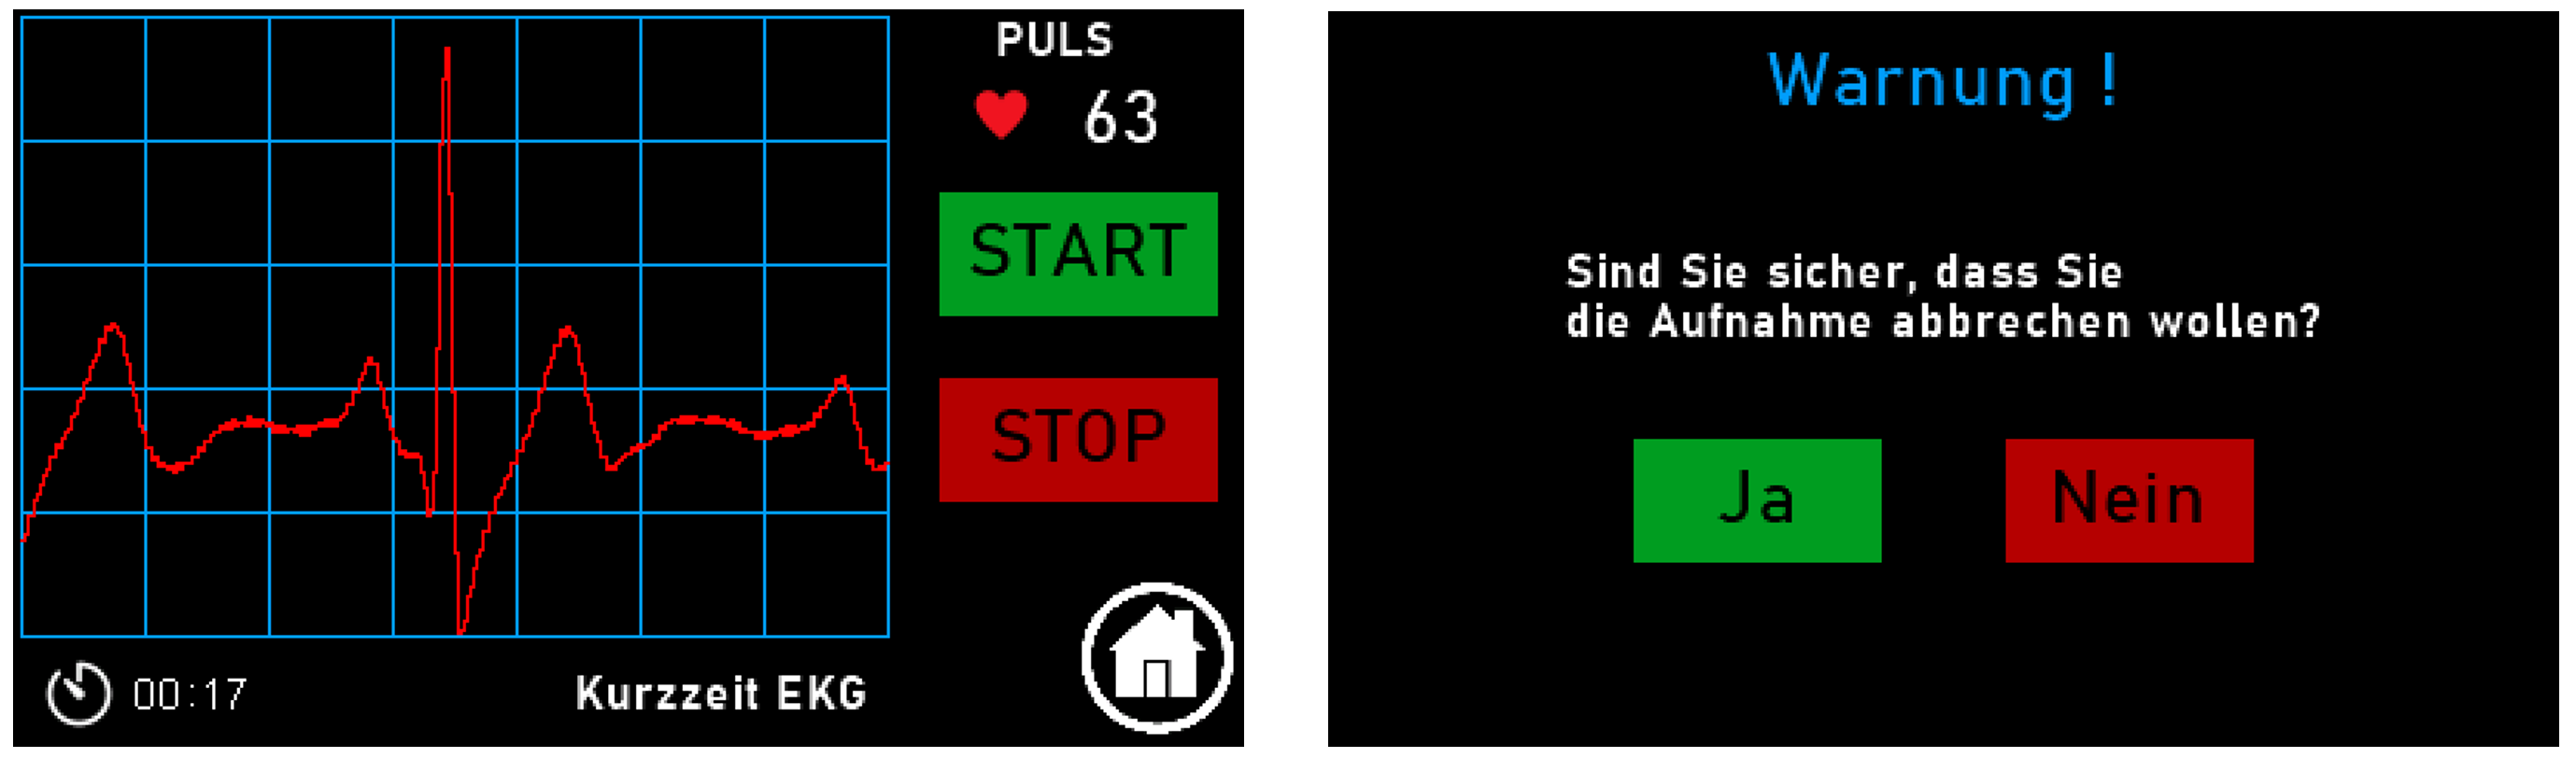
\includegraphics[width=\textwidth] {Short ECG.png}
	\caption{Display UI einer Kurzzeit-Aufnahme}
\end{figure}

Im Kurzzeitmodus wird zudem kontinuierlich die Herzfrequenz gemessen und an das Display gesendet. Hierfür werden über einen Schwellwert die R-Zacken des Signals detektiert und die Anzahl der Werte zwischen diesen gezählt.

$$ Pulsfrequenz = \frac{\textit{Samples pro Minute}}{\textit{Samples zwischen zwei R-Zacken}} $$

Der Schwellwert wird permanent durch das Maximum und Minimum der vergangenen Signalperiode angepasst, um auf Schwankungen des Signals zu reagieren.

$$ Schwellwert = Minimum + 0,8 \cdot (Maximum - Minimum) $$

\subsubsection{Langzeit-EKG}

Während der Langzeit-Aufnahme werden die Daten auf der MCU gespeichert und alle vier Sekunden blockweise an die SD-Karte gesendet. Gestartet wird ebenfalls durch einen Start-Befehl auf dem Display. Hier ist jedoch zu beachten, dass der Ladestand beim Start mindestens 80 \% aufweisen muss, um eine EKG-Aufnahme über 24 Stunden zu gewährleisten. Wie im Kurzzeit-Modus kann der Benutzer den Kurvenverlauf und die Aufnahmedauer am Display ansehen. 

Durch Betätigen des Tasters wird der Energiesparmodus aktiviert. Die Logik des Stromsparmodus enthält eine weitere \textit{State Machine} mit drei Zuständen. Die State Machine ist mit einer switch-Anweisung realisiert. Die drei Zustände sind: normaler Zustand \textit{(MODE\_NORMAL)}, 5V Peripherie an \textit{(MODE\_5V\_ON)} und 5V Peripherie aus \textit{(MODE\_5V\_OFF)}. Das Funktionsprinzip des Energiesparmodus ist auf dem Bild zu sehen.

\begin{figure} [!h]
    \centering
    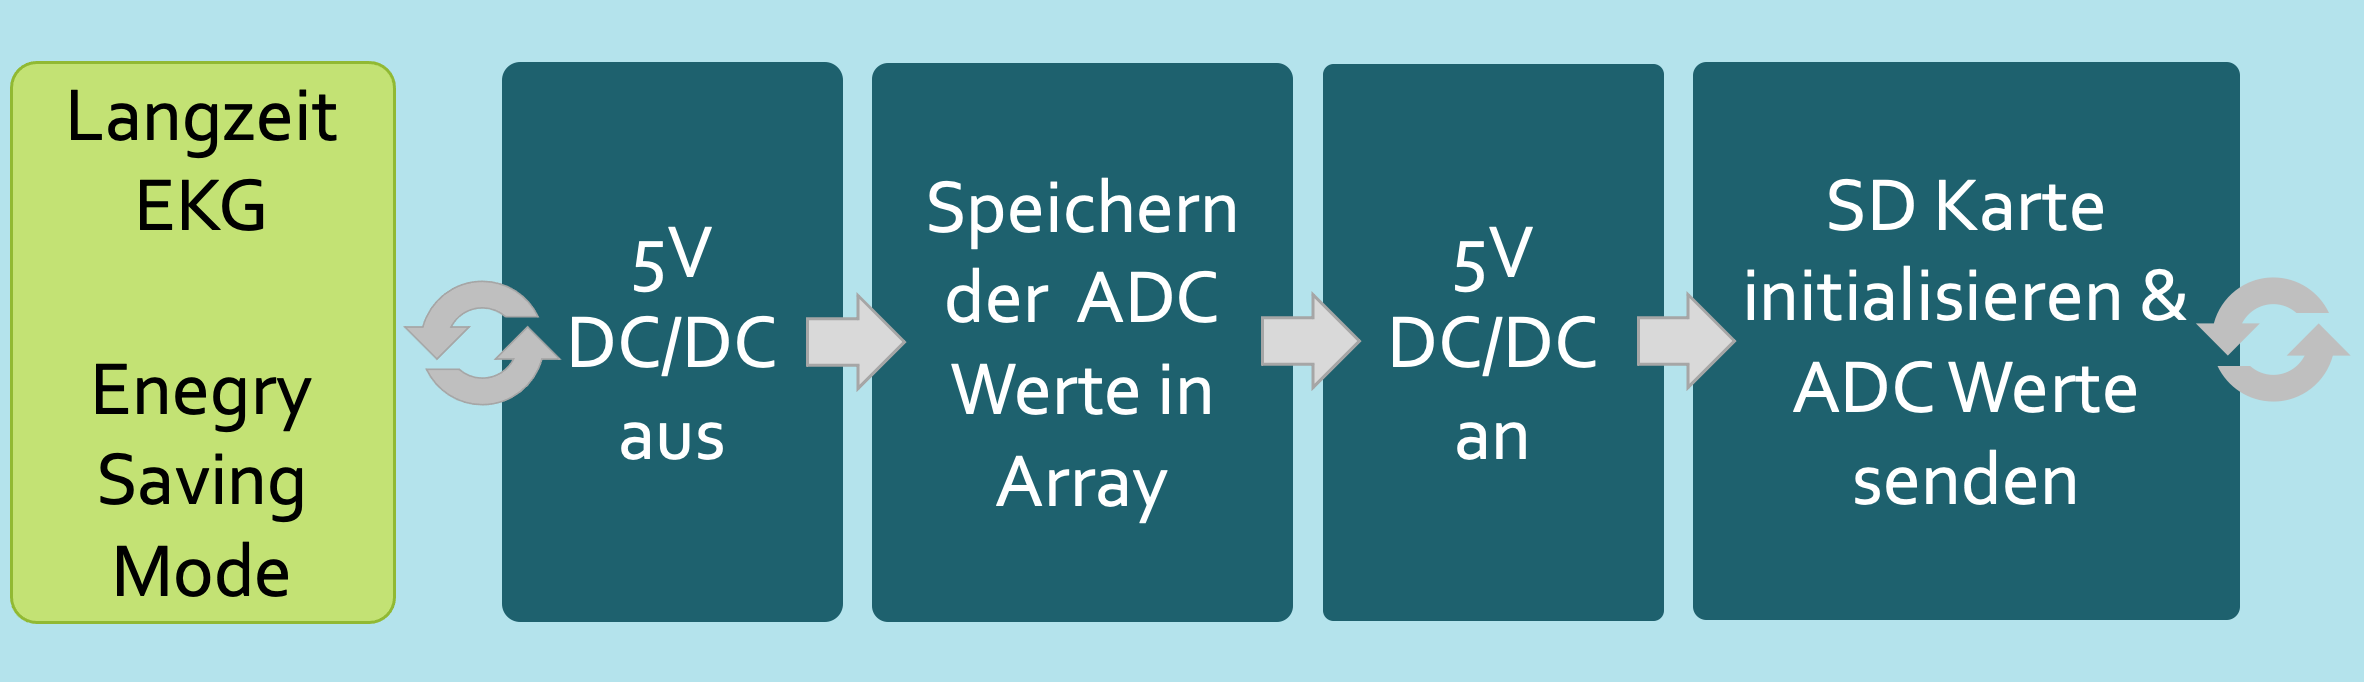
\includegraphics[width=12cm] {Langzeit EKG Energy Saving.png}
    \caption{Energy Saving Mode während Langzeit-EKG}
\end{figure}

Im normalen Zustand bleibt die ganze 5V Peripherie angeschaltet. Der Kurvenverlauf ist auf dem Display zu sehen. Der einzige Unterschied ist das Schreiben auf die SD-Karte. Dieser Vorgang ist folgendermaßen realisiert. Es sind zwei Arrays mit jeweils 1000 Werten benutzt. Da der ADC am 250Hz-Timer gebunden ist, wird dieses Array innerhalb von 4 Sekunden aufgefüllt. Um sie zu unterscheiden, werden sie Main Storage und Redundant Storage genannt. Im ADC Interrupt wird jeder neue ADC-Wert in Main Storage gespeichert, und zwar so lange, bis das Array voll wird. Nachdem das Main Storage voll ist, wird das ganze Array in Redundant Storage kopiert. Somit kann Main Storage wieder überschrieben werden und währenddessen bleibt Redundant Storage unverändert. Wenn Main Storage voll ist und in Redundant Storage kopiert, wird eine \textit{Flag} gesetzt und somit das Senden an die SD-Karte gestartet. Nachdem das Senden fertig ist, wird der ganze Vorgang wiederholt.
Wenn der Taster betätigt wird, geht die MCU aus dem Zustand \textit{MODE\_NORMAL} in den \textit{MODE\_5V\_OFF}. In diesem Zustand wird die 5V Peripherie abgeschaltet. Der Zustand kann verlassen werden, wenn entweder Main Storage voll ist und die entsprechende \textit{Flag} gesetzt ist, oder der Taster erneut betätigt wird.
Wenn die \textit{Flag} gesetzt wird, geht die MCU in den Zustand \textit{MODE\_5V\_ON}, in dem die 5V Peripherie wieder versorgt wird. Demnächst wird die SD-Karte initialisiert und das bereits kopierte Redundant Storage an die SD-Karte geschrieben. Danach geht die MCU in den Zustand \textit{MODE\_5V\_OFF} und der Vorgang wird wiederholt.
Wenn der Taster betätigt wird, geht die MCU in den Zustand \textit{MODE\_NORMAL} und zeigt die Werte auf dem Display an. In diesem Zustand kann der Benutzer das Gerät wieder in den Energiesparmodus versetzen oder die Aufnahme vorzeitig beenden. Für das beenden, kann der Stopp-Button auf dem Display betätigt werden. Wie auch beim Kurzzeit-EKG wird durch die Sicherheitsabfrage ein unbewusstes Drücken verhindert. Die Aufnahme wird ansonsten nach 24 Stunden automatisch beendet. Die MCU gelangt dann zurück in den Idle Zustand.

\subsubsection{Energy Saving Mode und Wakeup Mode}

Um die Batterielaufzeit bei einer Lagerung zu verlängern, verfügt das EKG-Gerät über einen Energiesparmodus. Wenn das Gerät eingeschaltet ist und sich im \textit{IDLE\_STATE} befindet, kann der Taster am Gehäuse gedrückt werden. Dabei wird in den Zustand \textit{ENERGY\_SAVING\_MODE} gewechselt. Dieser schaltet den 5 V DC/DC und die damit verbundene Peripherie ab. Beim Ausschalten ist ein akustisches Signal eines Buzzers zu hören. Die Überwachung des SD-Kartenstatus läuft über 3 V. Daher ist diese selbst im \textit{ENERGY\_SAVING\_MODE} vorhanden. Sollte die SD-Karte währenddessen entfernt werden, wird eine SD-\textit{Flag} im GPIO gesetzt.
Wenn im Energiesparmodus der Taster am Gehäuse erneut betätigt wird, gelangt man in den Zustand \textit{SYS\_WAKEUP}. In diesem Zustand wird die 5 V Peripherie wieder angeschaltet und das akustische Signal des Buzzers ist zu hören. Sollte die SD-Karte während dem Energiesparmodus entfernt worden sein, wird der Benutzer auf dem Display darauf hingewiesen. Sollte die SD-Karte nun erneut eingesteckt werden, erfolgt eine Initialisierung und das SD-Karten Symbol auf dem Display wird aktualisiert.
Das EKG-Gerät befindet sich schließlich wieder im \textit{IDLE\_STATE}.

Die Logik wird Anhand der Abbildung \ref{fig. energysavingmode} verdeutlicht.

\begin{figure} [!h]
	\centering
	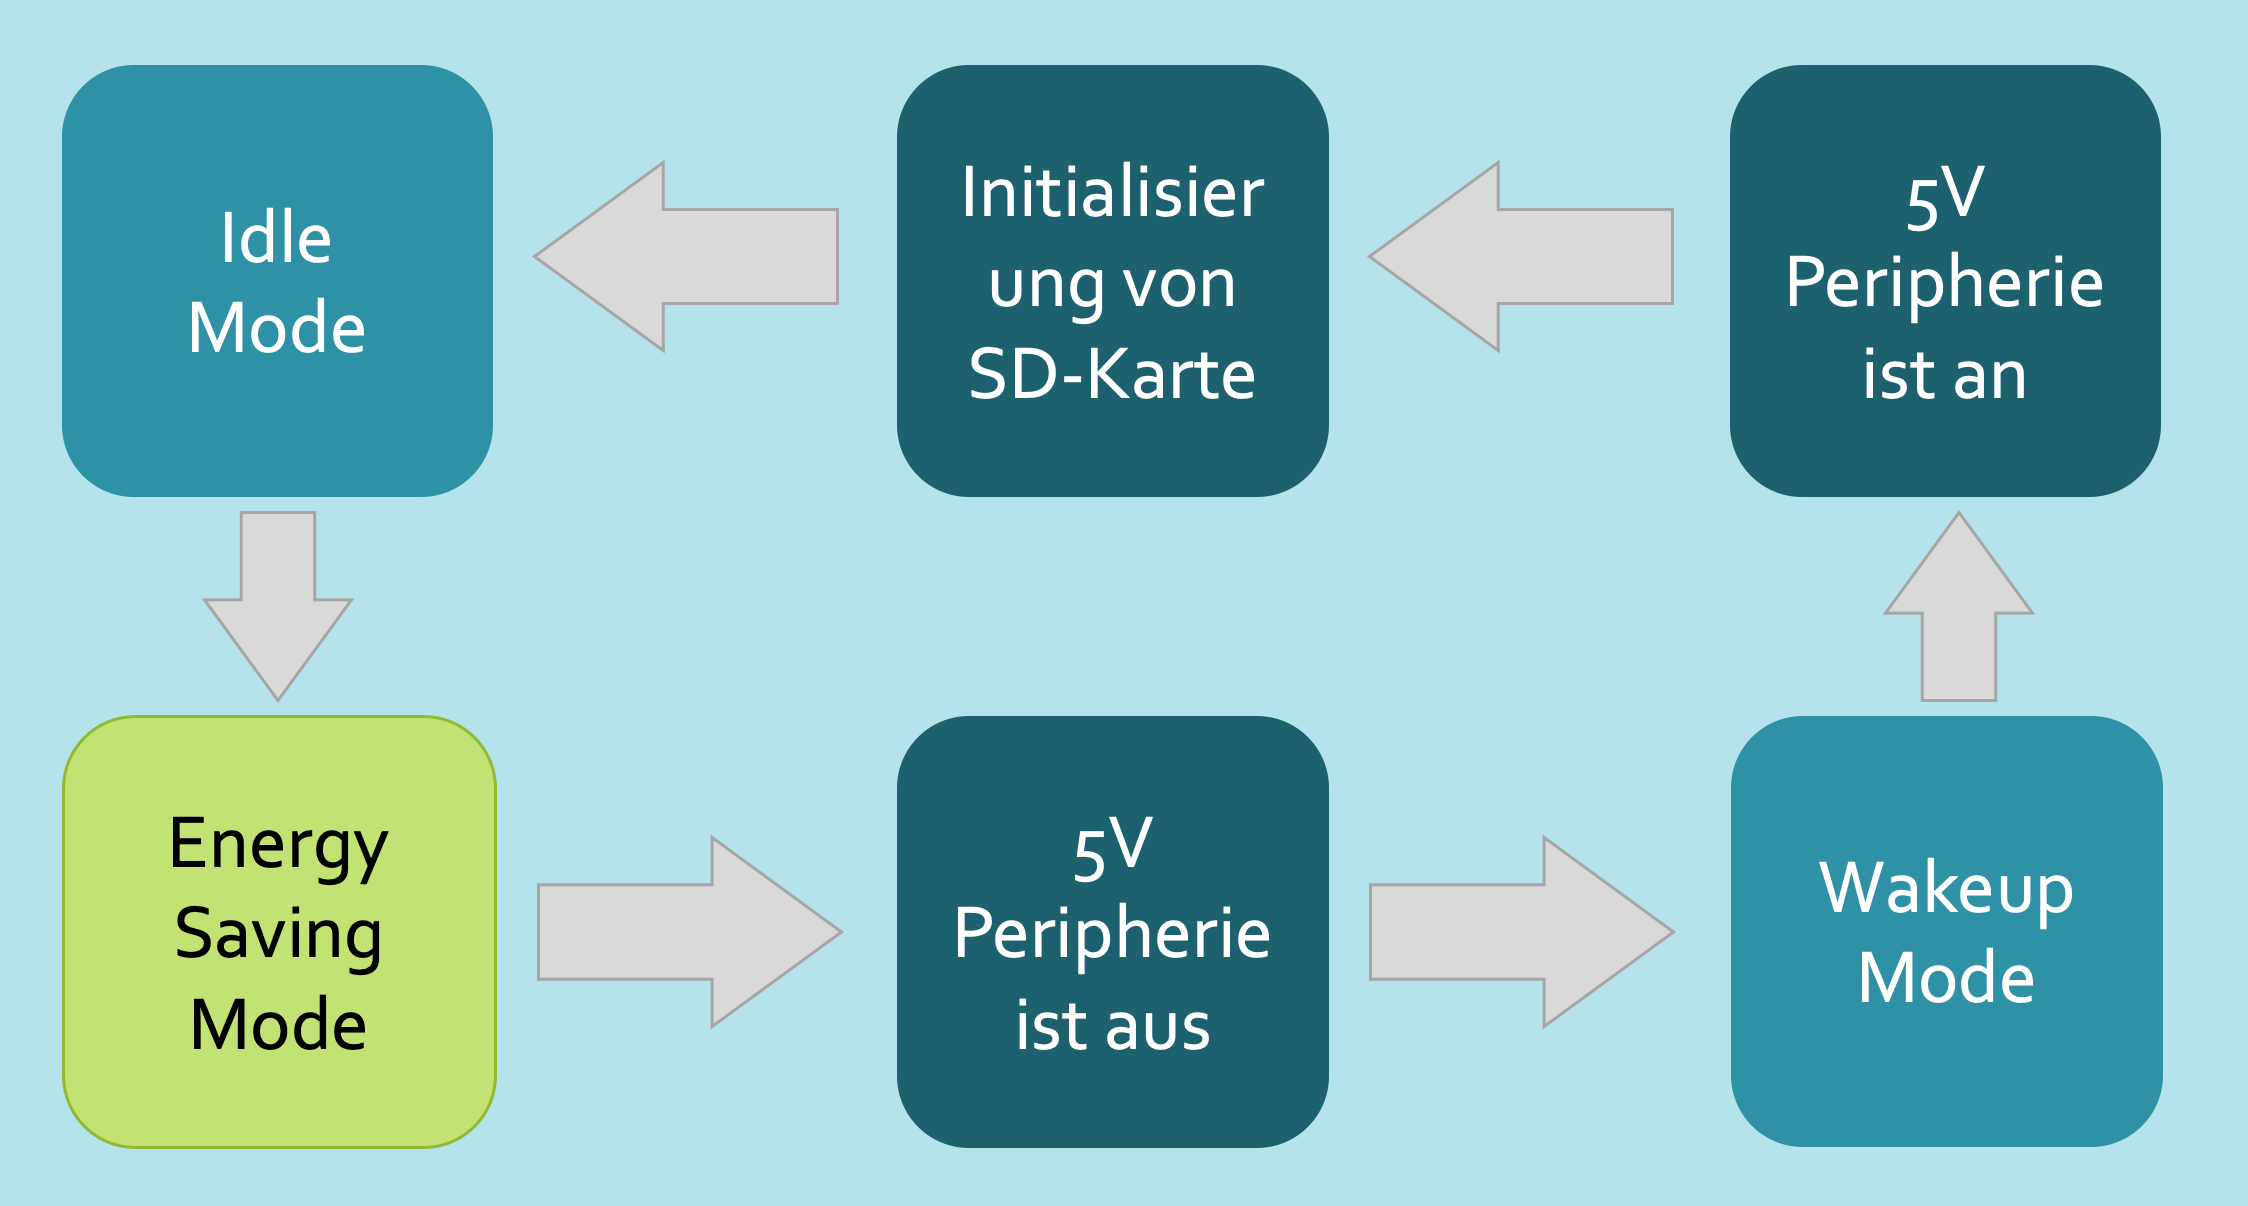
\includegraphics[width=12cm] {Idle State and Evergy Saving.png}
	\caption{Energy Saving Mode in Idle State}
    \label{fig. energysavingmode}
\end{figure}

\subsubsection{Akku-, BT-, SD-Abfrage}

Ausßerhalb der switch-Anweisung, die die \textit{State Machine} bildet, werden jede Sekunde folgende Funktionen aufgerufen.
\begin{itemize}
    \item \textit{ADC\_Akku\_Average\_Value} berechnet über drei Sekunden den Mittelwert der ADC-Werte der Akkuspannung. Diese werden als Information für den Benutzer an das Display gesendet.
    \item \textit{Check\_BT\_Connection} und \textit{Check\_SD\_Card\_Connection} sind zwei Funktionen, die die aktuelle Verbindung der Peripherie zum Bluetooth Modul und zum SD-Kartenleser ermitteln und auf dem Display anzeigen. Hierfür werden die State-Pins der Module abgefragt. Besteht eine Verbindung zum jeweiligen Modul, sind die Symbole auf dem Display blau, anderenfalls sind die grau. Der Start einer Langzeitaufnahme ist nur mit angeschlossener SD-Karte möglich.
    Bei der Abfrage für die SD-Karte gibt es außerdem zwei zusätzliche Funktionen. Wenn die SD-Karte herausgezogen wird, erscheint auf dem Display eine Warnmeldung. Beim Entfernen und wieder Anschließen einer SD-Karte, wird diese neu initialisiert und die aktuellen Daten bleiben vorhanden.
\end{itemize}

%\subsubsection{Aufnahme eines Kurzzeit-EKG}

%Die Kurzzeit-EKG-Aufnahme wird kontinuierlich durchgeführt. D.h. die ADC Werte werden direkt an das Display und SD-Karte übertragen ohne Zwischenspeichern. Nachdem die MCU auf ECG\_SHORT Zustand wechselt, wird als erstes ein Timer auf dem Display gestartet. Der Timer zählt, wie lange die EKG-Aufnahme durchgeführt wird. Nach zwei Minuten wird die Aufnahme automatisch beendet und der Benutzer wird benachrichtigt. Zunächst wird es auf 250 Hz \textit{Flag} gewartet und sobald die \textit{Flag} ungleich Null ist, wird ein ADC Wert aufgenommen und die \textit{Flag} wird zurückgesetzt. Wenn ein neuer ADC Wert ankommt, wird eine weitere \textit{Flag} gesetzt und dadurch wird der aufgenommene ADC Wert an das Display gesendet und demnächst auf die SD-Karte gespeichert. Die \textit{Flag} wird zurückgesetzt.
%Es wird durchgehend kontrolliert, dass es nur Kurzzeit-EKG aufgenommen wird. Sollte der Benutzer während der Aufnahme versuchen auf Langzeit-EKG zu wechseln, wird eine Warnung gezeigt und der Vorgang verhindert.
%Nach der Aufnahme wird die \textit{Flag} für Kurzzeit-EKG zurückgesetzt, die Datei auf der SD-Karte gespeichert, die Timer zurückgesetzt und die MCU geht in Idle Zustand. Das Display wird dementsprechend die Hauptseite anzeigen.

%Im Kurzzeitmodus wird zudem kontinuierlich die Herzfrequenz gemessen und an das Display gesendet. Hierfür werden über einen Schwellwert die R-Zacken des Signals detektiert und die Anzahl der Werte zwischen diesen gezählt. 

%$ Pulsfrequenz = \frac{Maximalanzahl der Werte in einer Minute}{Anzahl der Werte einer Signalperiode} $

%Der Schwellwert wird permanent durch das Maximum und Minimum der vergangenen Signalperiode angepasst, um auf Schwankungen des Signals zu reagieren.

%$ Schwellwert = Minimum + 0,8 * (Maximum - Minimum) $

%\subsubsection{Aufnahme eines Langzeit-EKG}

%Im Gegensatz zu Kurzzeit-EKG, werden die Daten während der Langzeit-EKG-Aufnahme intern auf der MCU gespeichert und blockweise in gewissen Zeitintervallen an SD-Karte gesendet. Da das SD-Kartenmodul an 5V angeschlossen ist und im Stromsparmodus 5V Peripherie komplett abgeschaltet ist, weicht die Logik von Kurzzeit-Aufnahme ab.
%Beim Wechseln auf Langzeit-EKG Modus wird als erstes die Timer- und ADC-Werte an das Display gesendet. Somit kann der Benutzer den Kurvenverlauf und Dauer der Aufnahme sehen. Weiterhin wird die Stromsparmodus-Logik aufgerufen. Diese Logik enthält eine \textit{State Machine} mit drei Zuständen. Die State Machine ist mit einer switch-Anweisung realisiert. Die drei Zustände sind: normaler Zustand (MODE\_NORMAL), 5V Peripherie an (MODE\_5V\_ON) und 5V Peripherie aus (MODE\_5V\_OFF). 
%Die zwei Modi für 5V an und aus sind für Stromsparmodus entwickelt. Das Funktionsprinzip des Stromsparmodus ist auf dem Bild zu sehen.
%\begin{figure} [!h]
%	\centering
%	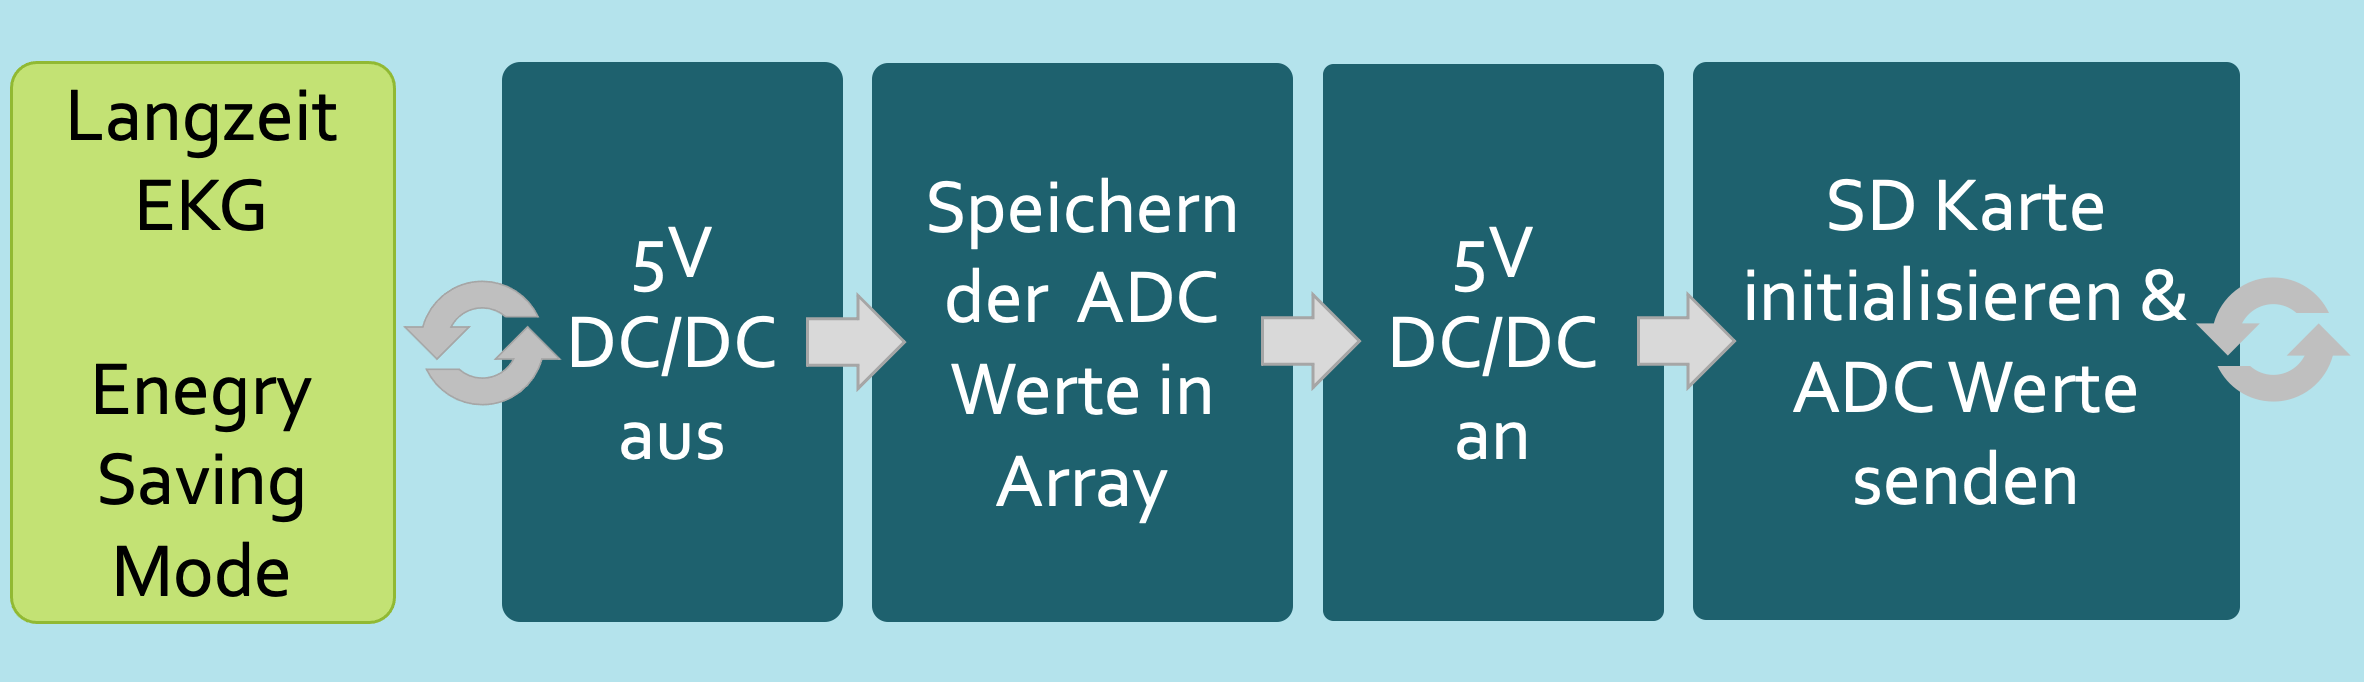
\includegraphics[width=12cm] {Langzeit EKG Energy Saving.png}
%	\caption{Energy Saving Mode während Langzeit-EKG}
%\end{figure}
%Wenn der Benutzer 24 Stunden Aufnahme macht, ist es sinnvoll Energie zu sparen. Im Stromsparmodus wird die ganze 5V Peripherie komplett abgeschaltet, d.h. das Display, Bluetooth und SD-Karte werden nicht mehr versorgt. Das Stromsparmodus kann aktiviert werden, wobei der Benutze den Power Button auf dem Gehäuse einmal betätigt.
%Wenn der Benutzer eine Langzeit-EKG-Aufnahme gestartet hat, landet das Programm in MODE\_NORMAL zuerst und bleibt in diesem Zustand solange, bis der Benutzer den Power Button betätigt. Im normalen Zustand bleibt die ganze 5V Peripherie an, das QRS Komplex ist auf dem Display zu sehen und die ADC-Werte werden via Bluetooth gesendet. Der einzige Unterschied ist das Schreiben auf SD-Karte. Dieser Vorgang ist komplett verarbeitet und ist folgendermaßen realisiert. Es sind zwei Arrays mit jeweils 1000 Werten benutzt. Dadurch, dass ADC an 250Hz Timer gebunden ist, wird dieses Array innerhalb von 4 Sekunden aufgefüllt. Um sie zu unterscheiden, werden sie Main Storage und Redundant Storage genannt. Im ADC Interrupt wird jeder neue ADC-Wert in Main Storage gespeichert, und zwar so lange, bis das Array voll wird. Nachdem das Main Storage voll ist, wird das ganze Array in Redundant Storage kopiert. Somit kann Main Storage wieder überschrieben werden und währenddessen bleibt Redundant Storage unverändert. Wenn Main Storage voll ist und in Redundant Storage kopiert, wird eine \textit{Flag} gesetzt und somit das Senden an SD-Karte gestartet. Nachdem das Senden fertig ist, wird der ganze Vorgang wiederholt.
%Wenn der Power Button betätigt wird, geht die MCU aus dem MODE\_NORMAL in MODE\_5V\_OFF. In diesem Zustand wird 5V Peripherie abgeschaltet. Der Zustand kann verlassen werden, wenn entweder Main Storage voll ist und entsprechende \textit{Flag} gesetzt ist, oder der Power Button nochmal betätigt wird.
%Wenn die \textit{Flag} gesetzt wird, geht die MCU in MODE\_5V\_ON in dem die 5V Peripherie wieder versorgt wird. Demnächst wird die SD-Karte initialisiert und das bereits kopierte Redundant Storage an die SD-Karte geschrieben. Danach geht die MCU in MODE\_5V\_OFF und der Vorgang wird wiederholt.
%Wenn der Power Button betätigt wird, geht die MCU in MODE\_NORMAL, zeigt die Werte auf dem Display und sendet Daten via Bluetooth bei Bedarf. In diesem Zustand kann der Benutzer entweder die Aufnahme beenden oder das Gerät wieder in Energy Saving Mode senden. 
%Die Aufnahme wird nach 24 Stunden automatisch beendet und die MCU geht wieder in Idle State.

